\fancyhead[LE]{\fontsize{8.5pt}{10pt}\selectfont\textbf{\textsf{\thepage}}\quad \textbf{\textsf{CHƯƠNG 1}}\quad \textsf{Các hàm số và Mô hình}}
\fancyhead[RO]{\fontsize{8.5pt}{10pt}\selectfont\textsf{MỤC 1.2}\quad \textsf{Mô hình Toán học: Danh mục các Hàm số Cơ bản}\quad \textbf{\textsf{29}}}

\noindent
\begin{minipage}[t]{0.265\textwidth}
    \fontsize{8pt}{10pt}\selectfont
    \vspace*{285pt}
    \begin{center}
        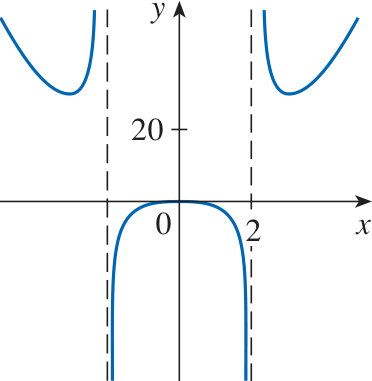
\includegraphics[width=0.92\linewidth]{images/p0064_fig18.png}\\[4pt]
        {\raggedright\textbf{\textsf{HÌNH 18}}\\[2pt]
        $f(x) = \dfrac{2x^4 - x^2 + 1}{x^2 - 4}$\par}
    \end{center}
\end{minipage}%
\hfill
\begin{minipage}[t]{0.708\textwidth}
    \fontsize{9.3pt}{13.2pt}\selectfont
    \noindent trong đó $C$ là một hằng số. Do đó đồ thị của $I$ như một hàm số theo $x$ (xem Hình 17) có hình dạng chung tương tự như nửa bên phải của Hình 16.

    \vspace{0.5em}
    \noindent
    \begin{minipage}[t]{0.48\linewidth}
        \centering
        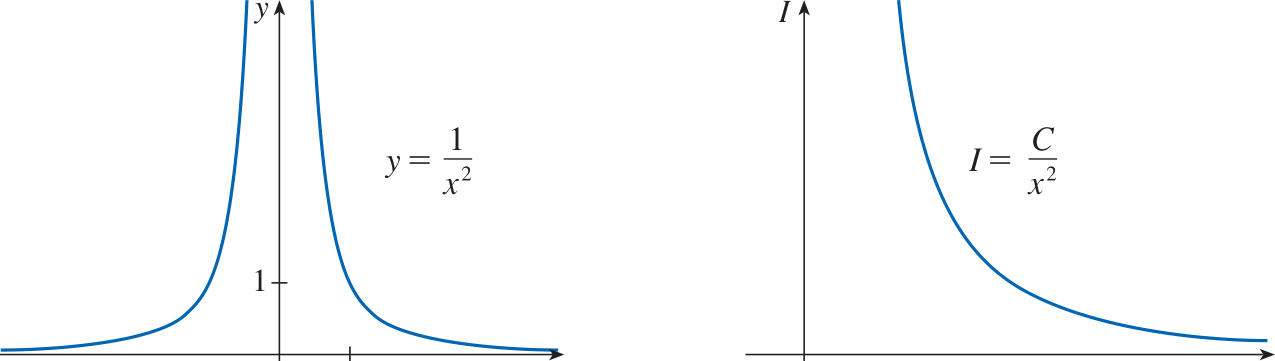
\includegraphics[width=\linewidth]{images/p0064_fig16.png}\\[4pt]
        {\raggedright\fontsize{8pt}{10pt}\selectfont
        \textbf{\textsf{HÌNH 16}}\\
        Nghịch đảo của hàm bình phương\par}
    \end{minipage}\hfill
    \begin{minipage}[t]{0.48\linewidth}
        \centering
        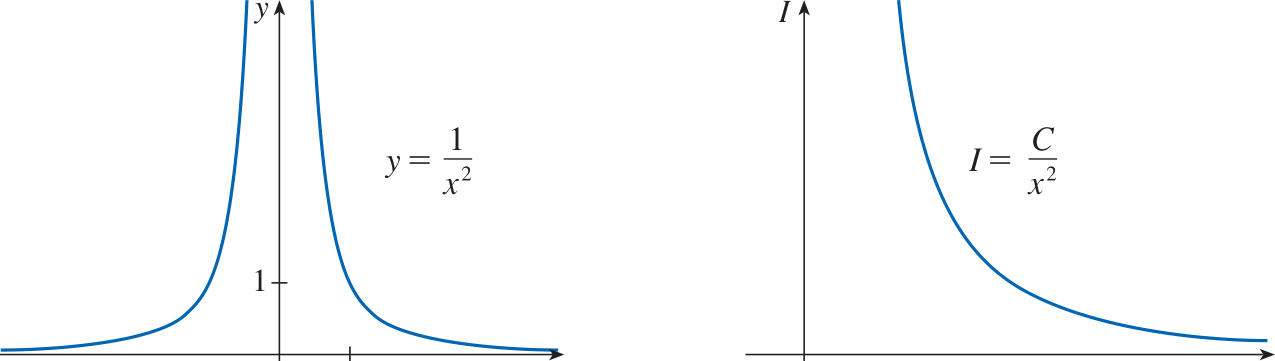
\includegraphics[width=\linewidth]{images/p0064_fig17.png}\\[4pt]
        {\raggedright\fontsize{8pt}{10pt}\selectfont
        \textbf{\textsf{HÌNH 17}}\\
        Độ rọi từ một nguồn sáng theo khoảng cách từ nguồn\par}
    \end{minipage}

    \vspace{1em}
    Các định luật nghịch đảo bình phương mô hình hóa lực hấp dẫn, độ to của âm thanh và lực tĩnh điện giữa hai hạt mang điện. Xem Bài tập 37 để biết lý do hình học giải thích tại sao các định luật nghịch đảo bình phương thường xuất hiện trong tự nhiên.

    Các hàm lũy thừa cũng được sử dụng để mô hình hóa mối quan hệ giữa số lượng loài và diện tích (Bài tập 35--36) và chu kỳ quay của một hành tinh như một hàm số theo khoảng cách của nó tới Mặt Trời (xem Bài tập 34).

    \vspace{1em}
    \noindent{\color{stewartcyan}\rule{1.1ex}{1.1ex}}\hspace{0.5em}\textbf{\textsf{Hàm hữu tỉ}}
    \vspace{0.4em}

    \noindent Một \textbf{hàm hữu tỉ} $f$ là tỉ số của hai đa thức:
    \begin{equation*}
    f(x) = \frac{P(x)}{Q(x)}
    \end{equation*}
    trong đó $P$ và $Q$ là các đa thức. Tập xác định gồm tất cả các giá trị của $x$ sao cho $Q(x) \neq 0$. Một ví dụ đơn giản về hàm hữu tỉ là hàm $f(x) = 1/x$, có tập xác định là $\{x \mid x \neq 0\}$; đây là hàm nghịch đảo có đồ thị được vẽ trong Hình 14. Hàm số
    \begin{equation*}
    f(x) = \frac{2x^4 - x^2 + 1}{x^2 - 4}
    \end{equation*}
    là một hàm hữu tỉ với tập xác định $\{x \mid x \neq \pm 2\}$. Đồ thị của nó được thể hiện trong Hình 18.

    \vspace{1em}
    \noindent{\color{stewartcyan}\rule{1.1ex}{1.1ex}}\hspace{0.5em}\textbf{\textsf{Hàm đại số}}
    \vspace{0.4em}

    \noindent Một hàm số $f$ được gọi là một \textbf{hàm đại số} nếu nó có thể được xây dựng bằng cách sử dụng các phép toán đại số (như phép cộng, trừ, nhân, chia và khai căn) bắt đầu từ các đa thức. Mọi hàm hữu tỉ đều đương nhiên là một hàm đại số. Dưới đây là hai ví dụ khác:
    \begin{equation*}
    f(x) = \sqrt{x^2 + 1} \qquad g(x) = \frac{x^4 - 16x^2}{x + \sqrt{x}} + (x - 2)\sqrt[3]{x + 1}
    \end{equation*}
    Trong Chương 4, chúng ta sẽ khảo sát và phác họa đồ thị của nhiều hàm đại số khác nhau, và chúng ta sẽ thấy rằng đồ thị của chúng có thể mang rất nhiều hình dạng đa dạng.
\end{minipage}